\documentclass[12pt,a4paper]{article}
\usepackage{amssymb, amsmath}
\usepackage{theorem}
\usepackage{clrscode}
\usepackage{fullpage}
\usepackage{graphicx}
\usepackage{enumitem}

\setlength{\parskip}{0cm}
\setlength{\parindent}{0pt}
\newtheorem{thm}{Theorem}

\renewcommand{\thesubsubsection}{\arabic{subsubsection})}

\pagestyle{empty}

\begin{document}

\begin{center}
  
  \bigskip \bigskip

  {\huge \textbf{Machine Learning}}

  \bigskip
  
  {\large Spring 2020}

  \bigskip \bigskip

  {\large \textsc{Homework 1}} 
  
  \bigskip \bigskip
  
  {\large \textbf{Ozren Dabić}}
  
  \bigskip \bigskip

\end{center}

\section*{Questions}

\subsection*{Training versus Validation}

\begin{figure}[h!]
\begin{center}    
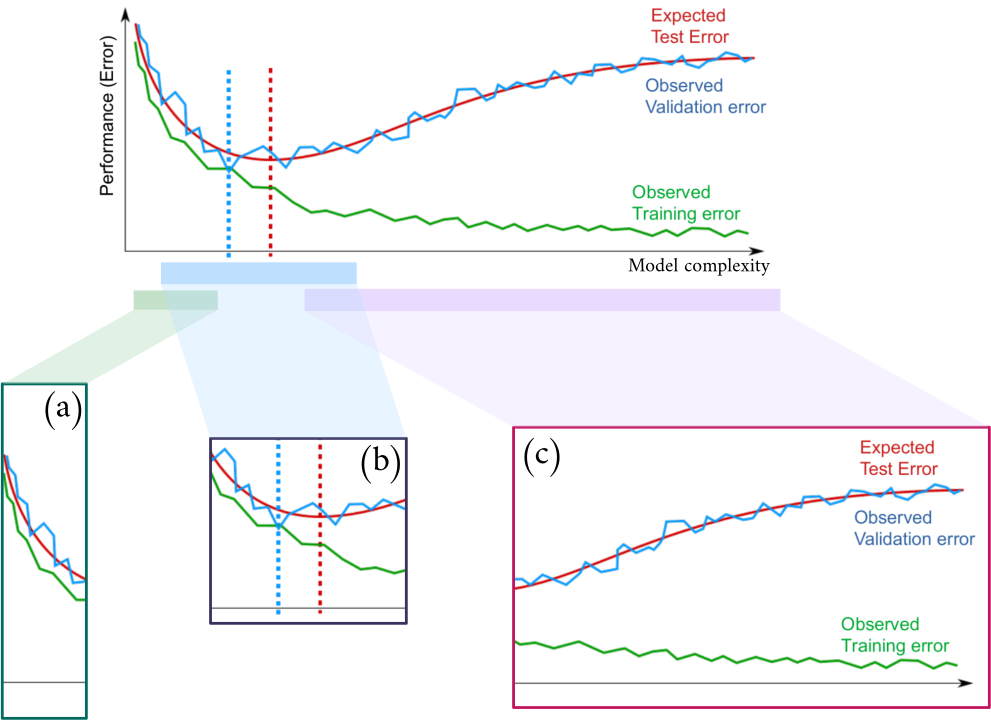
\includegraphics[height=0.7\textwidth,keepaspectratio]{figures/figure1}
\end{center}
\caption{This is what you missed last class}
\end{figure}

\subsubsection*{What is the whole figure about?}

This figure represents the relationship between the approximation performance and model complexity of a linear regression model.

\subsubsection*{Explain the curves' behaviour in each of the three highlighted sections of the figures!}

First let's explain what each of the curves represents. When training our linear regression model, we spit our data into 3 sets: the training, validation and test set. The training set is used exclusively to train the model, while the test set is used to determine accuracy of said training. The validation set is used to determine how well the model generalises unseen data. Observing the graph, we notice that the error of all 3 performance measures is high when model complexity is low. The model simply has not trained enough to make accurate predictions for either seen or unseen data. As model complexity increases, so does the accuracy of the model. Two vertical lines are observable in this section. They represent the optimal models, according to the validation and test set respectively. As model complexity increases further, the training set performance increases, but the validation and test set performance decrease. This is because the model is overtrained to generalise data according to the training set, preventing it from making correct generalisations when being fed the (unseen) validation data.

\subsubsection*{Is any of the three section associated with the concepts of overfitting and underfitting?}

\begin{enumerate}[label=\alph*)]
\itemsep-0.25em 
	\item This section illustrates the consequence of a model suffering from underfitting. Due to a lack of training, underfit models can not accurately model the training data. As a result, regression never picks up the trend present in the data, leading to unreliable predictions.
	\item An optimal model, is a model that generalises well. Such a model is neither underfit nor overfit. This section represents an optimal model of our validation set and test set, both lines pointing to the exact model complexity required for the two sets to be considered optimal.
	\item While section a) was dedicated to underfitting, this final section displays the case of overfitting. While a lack of training can negatively effect predictions, too much training can also have a negative impact. Overfitting occurs in such a case, when a model learns the training data too well, leading to unreliable generalisations (hence the huge performance disparity between the observed training error and the validation/test error). The purpose of regression is to capture and fit the data according to a dominant trend, not according to all trends.
\end{enumerate}

\subsubsection*{What is early stopping?}

Early stopping is a method for controlling model complexity, with the central goal of avoiding overfitting. Early stopping rules provide guidance as to how many iterations can be run before the learner begins to over-fit. To find this ideal number of iterations, one must observe when the training set error begins to deviate from the validation set error, as the deviation is a clear sign of a model entering the overfitting stage.

\subsection*{Linear Regression}

\subsubsection{}

By introducing $x_3 = x_1 + 0.2 * x_2$ to our regression model:

\begin{equation*}
	f(x,\theta) = \theta_0 + \theta_1 * x_1 + \theta_2 * x_2
\end{equation*}

We obtain:

\begin{equation*}
	f(x,\theta) = \theta_0 + \theta_1 * x_1 + \theta_2 * x_2 + \theta_3 * x_3
	=
	\theta_0 + \theta_1 * x_1 + \theta_2 * x_2 + \theta_3 * (x_1 + 0.2 * x_2)
\end{equation*}

Which through several permutations finally yields:

\begin{equation*}
	f(x,\theta) =
	\theta_0 + (\theta_1 + \theta_3) * x_1 + (\theta_2 + 0.2 * \theta_3) * x_2
\end{equation*}

From this we can conclude that by introducing the regressor $x_3$

\subsubsection{}

\subsubsection{}

\end{document}
